% ============================================================================
\chapter{데이터셋}\label{ch:dataset}
% ============================================================================

본 연구는 서로 다른 기관과 장비에서 수집된 두 공개 데이터셋, TN3K와 DDTI를 함께 사용한다.
두 데이터셋을 의도적으로 혼합한 이유는 \secref{sec:problem}의 P2, 즉 데이터셋 간 이질성을 학습과 평가에
모두 반영하기 위해서이다. 이 장에서는 각 데이터셋의 특성(\secref{sec:ds_tn3k}, \secref{sec:ds_ddti}),
두 데이터셋의 정량적 차이(\secref{sec:ds_gap}), 전처리 절차(\secref{sec:ds_preproc}),
그리고 분할 설계(\secref{sec:ds_split})를 설명한다.

\section{TN3K}\label{sec:ds_tn3k}

TN3K\citep{gong2021multitask,gong2023trfe}는 갑상선 결절 초음파 영상 3,493장과 픽셀 단위 결절 마스크로
구성된 데이터셋이다. 배포 시 학습·검증용 2,879장과 평가용 614장으로 나뉘어 있으며, 본 연구는 이 구분을
그대로 따라 평가용 614장을 어떤 학습이나 모델 선택에도 사용하지 않는 held-out 집합으로 두었다.

\figref{fig:tn3k_samples}에서 보듯 TN3K 영상은 결절 주변을 잘라낸 확대 영상이 대부분이다.
그 결과 해상도가 184$\times$174부터 1463$\times$826까지 영상마다 제각각이며, 학습·검증 분할에서만
2,443종의 서로 다른 해상도가 나타난다. 판독 중 남긴 측정 커서(캘리퍼)가 영상에 그대로 찍혀 있는 경우도
있다. 한 영상에 결절이 둘 이상인 경우가 학습·검증 분할의 7.8\%, 평가 분할의 11.4\%를 차지한다.

\begin{figure}[htbp]
  \centering
  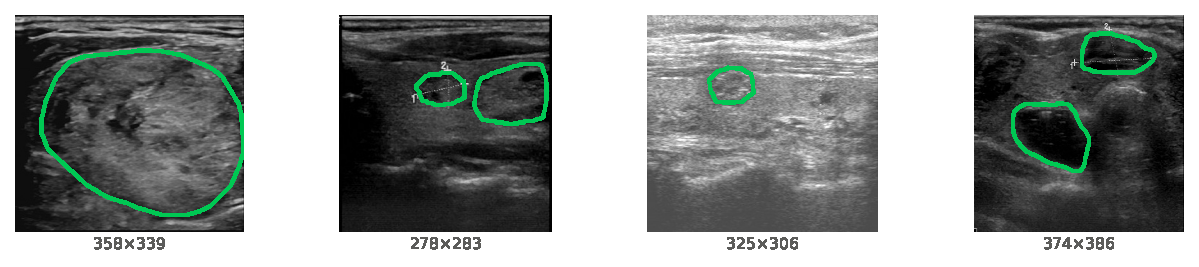
\includegraphics[width=\linewidth]{fig11_tn3k_samples}
  \caption[TN3K 표본과 정답 결절 경계(초록).]{TN3K 표본과 정답 결절 경계(초록). 각 영상 아래의 숫자는 원본 해상도이다.
    두 번째와 네 번째 영상에는 결절이 두 개씩 있다.}
  \label{fig:tn3k_samples}
\end{figure}

\section{DDTI}\label{sec:ds_ddti}

DDTI\citep{pedraza2015ddti}는 콜롬비아 IDIME 영상센터에서 수집한 갑상선 초음파 데이터셋이다.
본 연구에서는 결절 마스크가 제공되는 637장을 전부 학습·검증에 사용하였다.

DDTI 영상은 초음파 장비 화면을 그대로 캡처한 형태이다(\figref{fig:ddti_samples}). 그래서 영상 안에
게인 막대, 프로브 정보(P100, 12L6 등), 깊이 눈금, 좌우 표기(스페인어 DER·IZQ)가 함께 찍혀 있다.
높이는 모든 영상이 360 픽셀로 같고, 너비는 280, 560, 315, 245 픽셀의 네 종류뿐이다. 너비 560 픽셀 영상은
장비 화면 전체를, 280 픽셀 영상은 그중 초음파 영역 부근을 담고 있다. 637장 모두 결절이 정확히
하나씩이며, 다중 결절 사례는 하나도 없다.

\begin{figure}[htbp]
  \centering
  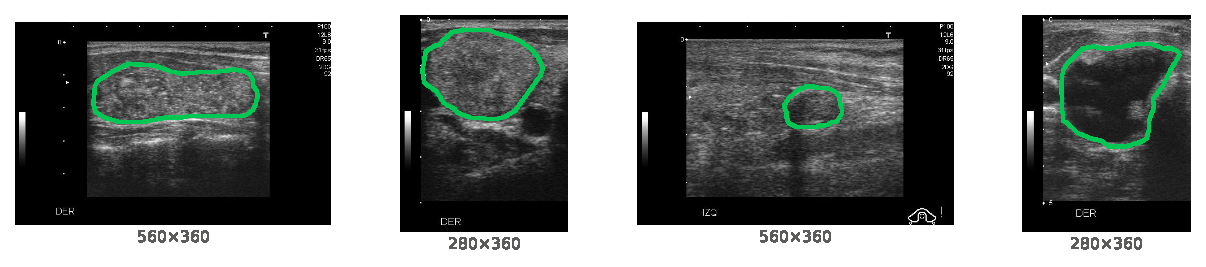
\includegraphics[width=\linewidth]{fig12_ddti_samples}
  \caption[DDTI 표본과 정답 결절 경계(초록).]{DDTI 표본과 정답 결절 경계(초록). 장비 화면의 게인 막대·눈금·좌우 표기가 영상에 포함되어 있다.}
  \label{fig:ddti_samples}
\end{figure}

\section{두 데이터셋의 정량적 차이}\label{sec:ds_gap}

\tabref{tab:dataset_stats}와 \figref{fig:dataset_stats}는 두 데이터셋의 차이를 정량적으로 보여 준다.
이 차이는 이후 교차 데이터셋 실험(\secref{sec:exp_lodo})의 설계 근거이자 그 결과를 해석하는 근거가 된다.

% 자동 생성 파일 — scripts/make_thesis.py 가 덮어쓴다. 직접 고치지 말 것.
\begin{table}[htbp]
\centering
\small
\caption[사용한 두 공개 데이터셋의 통계.]{사용한 두 공개 데이터셋의 통계. 결절 면적은 정답 폴리곤 면적을 영상 면적으로 나눈 값이다.}
\label{tab:dataset_stats}
\begin{adjustbox}{max width=\linewidth}
\begin{tabular}{lrrr}
\toprule
항목 & TN3K (trainval) & TN3K (test) & DDTI \\
\midrule
영상 수 & 2,879 & 614 & 637 \\
결절 수 & 3,130 & 690 & 637 \\
영상당 평균 결절 수 & 1.09 & 1.12 & 1.00 \\
결절 2개 이상 영상 비율 (\%) & 7.8 & 11.4 & 0.0 \\
파일 형식 & JPG & JPG & PNG \\
너비 범위 (px) & 184--1463 & 255--1399 & 245--560 \\
높이 범위 (px) & 174--826 & 261--772 & 360--360 \\
해상도 중앙값 (px) & 390$\times$336 & 436$\times$375 & 280$\times$360 \\
고유 해상도 종류 수 & 2,443 & 555 & 4 \\
결절 면적 중앙값 (영상 대비 \%) & 7.16 & 5.31 & 7.46 \\
결절 면적 5--95 백분위 (\%) & 0.88--42.95 & 0.59--37.33 & 1.52--23.76 \\
결절 면적 최솟값 (\%) & 0.056 & 0.162 & 0.524 \\
\bottomrule
\end{tabular}
\end{adjustbox}
\end{table}


\begin{figure}[htbp]
  \centering
  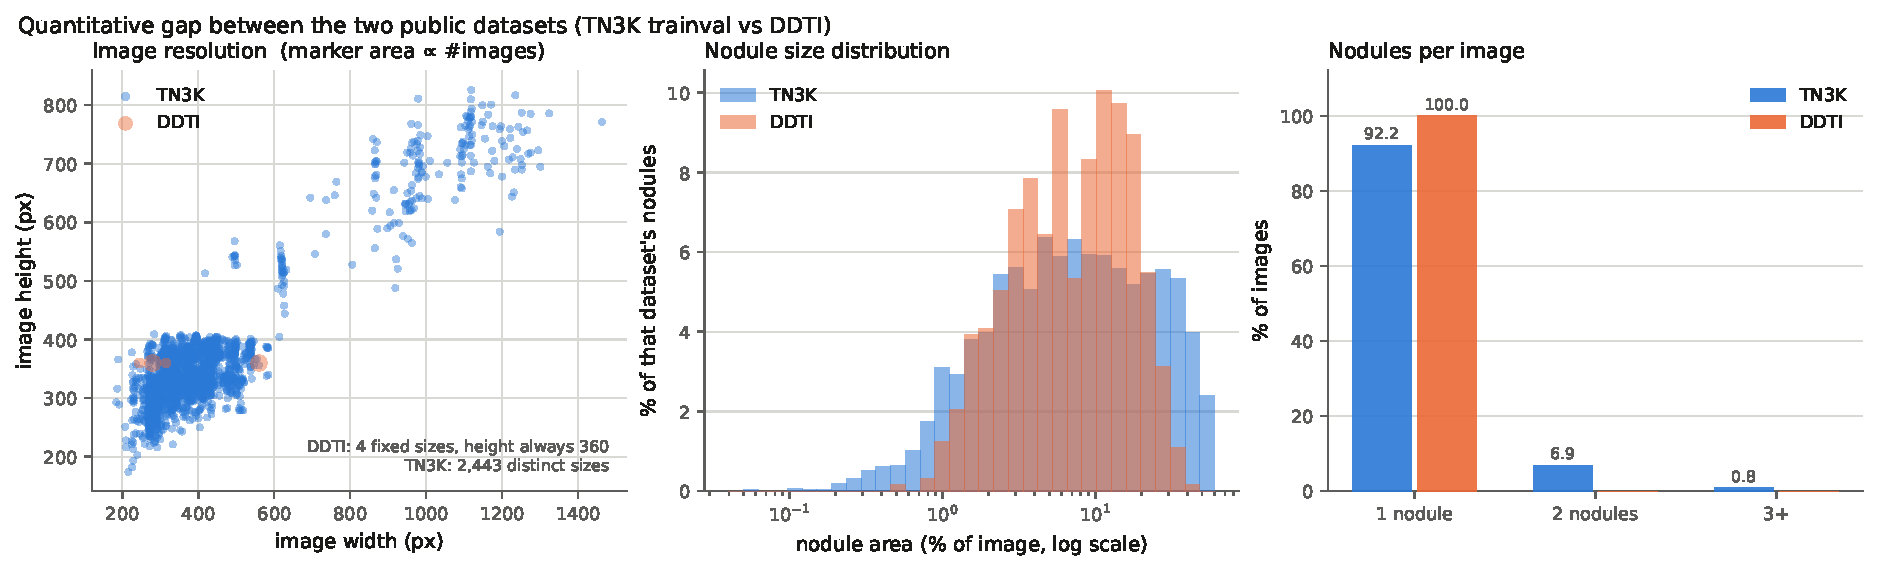
\includegraphics[width=\linewidth]{fig13_dataset_stats}
  \caption[두 데이터셋의 정량적 차이.]{두 데이터셋의 정량적 차이. (왼쪽) 영상 해상도 — 마커 넓이는 해당 해상도의 영상 수에 비례한다.
    (가운데) 결절 면적 분포 — 표본 수 차이를 없애기 위해 각 데이터셋 안에서의 비율로 정규화하였다.
    (오른쪽) 영상당 결절 수.}
  \label{fig:dataset_stats}
\end{figure}

\paragraph{해상도.} TN3K는 수천 종의 서로 다른 해상도를 가지는 반면 DDTI는 네 종류로 고정되어 있다.
학습 시에는 두 데이터셋 모두 640$\times$640 레터박스로 크기를 맞추지만, 원본에서 결절이 차지하는
픽셀 스케일의 분포는 크게 다르다.

\paragraph{결절 크기.} 결절 면적의 중앙값은 TN3K 7.16\%, DDTI 7.46\%로 비슷하지만 분포의 폭이 다르다.
TN3K는 영상의 0.06\%에 불과한 작은 결절부터 40\%를 넘는 큰 결절까지 넓게 퍼져 있는 반면, DDTI는
5--95 백분위가 1.52--23.76\%로 좁고 최솟값도 0.524\%이다. DDTI만으로 학습한 모델은 아주 작은 결절과
화면 대부분을 차지하는 큰 결절을 거의 본 적이 없다.

\paragraph{결절 수.} DDTI는 모든 영상이 단일 결절이다. DDTI로만 학습한 모델은 한 영상에 결절이 여럿 있는
장면을 학습하지 못하므로, TN3K로 옮겨 갔을 때 두 번째 결절을 놓칠 가능성이 높다.

\section{전처리}\label{sec:ds_preproc}

두 데이터셋은 정답을 비트맵 마스크로 제공한다. YOLOv11-seg는 객체마다 정규화된 다각형 좌표를 라벨로
받으므로, 마스크를 다각형으로 변환하였다. 두 데이터셋의 마스크는 JPEG 압축 잡음이 섞여 있거나
경계가 흐린 경우가 있어, 다음 절차를 두 데이터셋에 똑같이 적용하였다(\algref{alg:mask2poly}).

\begin{algorithm}[htbp]
\caption{정답 마스크의 YOLO-seg 다각형 변환}\label{alg:mask2poly}
\begin{algorithmic}[1]
\Require 마스크 영상 $M$ (높이 $h$, 너비 $w$)
\Ensure 정규화된 다각형 목록 $\mathcal{P}$
\State $B \gets [\,M > 127\,]$ \Comment{압축 잡음 제거를 위한 이진화}
\State $B \gets \mathrm{open}_{3\times3}(B)$ \Comment{모폴로지 열림으로 작은 잡티 제거}
\State $\mathcal{C} \gets$ 외곽 윤곽선 추출$(B)$ \Comment{내부 구멍은 무시}
\State $a_{\min} \gets \max(15,\ 0.0005\,hw)$
\For{각 윤곽선 $c \in \mathcal{C}$}
  \If{$\mathrm{area}(c) < a_{\min}$} \textbf{continue} \EndIf
  \State $c \gets$ Douglas--Peucker 단순화$(c,\ \varepsilon = 0.002 \cdot \mathrm{perimeter}(c))$
  \If{$|c| \ge 3$} $\mathcal{P} \gets \mathcal{P} \cup \{\, (x/w,\ y/h) \text{ for } (x,y) \in c \,\}$ \EndIf
\EndFor
\State \Return $\mathcal{P}$ \Comment{모든 다각형은 단일 클래스 `nodule'}
\end{algorithmic}
\end{algorithm}

최소 면적 기준(영상 면적의 0.05\%)은 마스크 잡티를 결절로 오인하지 않기 위한 것이다. 실제로 TN3K의 가장
작은 결절은 영상의 0.056\%로 이 기준을 넘는다. 변환 결과 TN3K 학습·검증 3,130개, TN3K 평가 690개,
DDTI 637개, 모두 4,457개의 결절 다각형을 얻었다. 변환된 다각형 전체를 원본 마스크 위에 겹쳐 그려
대조하였으며, 마스크가 있는데 라벨이 비거나 라벨이 누락된 영상은 없었다.

\section{분할 설계}\label{sec:ds_split}

실험의 목적에 따라 세 가지 분할을 구성하였다(\tabref{tab:splits}).

% 자동 생성 파일 — scripts/make_thesis.py 가 덮어쓴다. 직접 고치지 말 것.
\begin{table}[htbp]
\centering
\small
\caption[데이터 분할 구성.]{데이터 분할 구성. 괄호 안은 TN3K / DDTI 영상 수이다. pooled 5-fold의 평가는 모두 학습에 쓰이지 않은 TN3K test 614장에서 수행하였다.}
\label{tab:splits}
\begin{adjustbox}{max width=\linewidth}
\begin{tabular}{lrrrrr}
\toprule
분할 & 학습 & (TN3K / DDTI) & 검증 & (TN3K / DDTI) & 평가 \\
\midrule
fold 0 & 2,812 & 2,303 / 509 & 704 & 576 / 128 & 614 \\
fold 1 & 2,812 & 2,303 / 509 & 704 & 576 / 128 & 614 \\
fold 2 & 2,813 & 2,303 / 510 & 703 & 576 / 127 & 614 \\
fold 3 & 2,813 & 2,303 / 510 & 703 & 576 / 127 & 614 \\
fold 4 & 2,814 & 2,304 / 510 & 702 & 575 / 127 & 614 \\
\midrule
LODO TN3K$\rightarrow$DDTI & 3,493 & 3,493 / 0 & 637 & 0 / 637 & (= 검증, DDTI) \\
LODO DDTI$\rightarrow$TN3K & 637 & 0 / 637 & 3,493 & 3,493 / 0 & (= 검증, TN3K) \\
\bottomrule
\end{tabular}
\end{adjustbox}
\end{table}


\paragraph{Pooled 5-fold 교차검증.} TN3K 학습·검증 2,879장과 DDTI 637장, 합계 3,516장을 출처별로 따로
섞은 뒤(시드 42) 차례로 5개 fold에 배분하였다. 이렇게 하면 모든 fold의 검증 집합에서 TN3K와 DDTI의 비율이
전체 비율(약 82:18)과 같게 유지된다. 각 fold에서 학습은 약 2,812장, 검증은 약 704장이며, 검증 집합은
조기 종료와 체크포인트 선택에만 사용하였다.

\paragraph{Held-out 평가.} 모든 비교의 최종 평가는 TN3K 평가 분할 614장에서 수행하였다. 5개 fold에서
학습한 5개 모델을 각각 이 집합에서 평가하고, 결과를 fold 평균 $\pm$ 표준편차로 보고한다.

\paragraph{LODO (leave-one-dataset-out).} 한 데이터셋 전체로 학습하고 다른 데이터셋 전체에서 평가하여
도메인 일반화를 직접 측정한다. TN3K$\rightarrow$DDTI는 TN3K 3,493장(학습·검증·평가 분할 전부)으로 학습하고
DDTI 637장에서 평가하며, DDTI$\rightarrow$TN3K는 그 반대이다. 이 설정에서는 타깃 데이터셋을 검증 집합으로도
사용하므로, 체크포인트가 타깃 도메인 기준으로 선택된다. 두 모델이 같은 조건이므로 비교는 공정하지만,
보고되는 절대값은 실제 미지 도메인에서의 성능보다 낙관적일 수 있다(\secref{sec:limitations}).
